\documentclass[a4paper]{article}
\usepackage{lipsum}
\usepackage{url}
\usepackage{graphicx}
\usepackage{listings}
\usepackage{indentfirst}
\usepackage{enumerate}
\usepackage{multicol}
\lstset{language=Haskell}
\usepackage[margin=2cm]{geometry}
\graphicspath{ {images/} }
\renewcommand{\familydefault}{\sfdefault}

\title{COMP4075/G54RFP Coursework Part I}
\date{7\textsuperscript{th} November 2018}
\author{Benjamin Charlton - psybc3 - 4262648}

\usepackage{fancyhdr}

\pagestyle{fancy}
\fancyhf{}
\lhead{Benjamin Charlton | psybc3 | 4262648}
\rhead{G54RFP}
\cfoot{\thepage}

\begin{document}

\maketitle

\section{Task I.1 --- Hamming Numbers}
\subsection{Solutions}
For this problem I developed 2 solutions, one using a naive approach checking which numbers are hamming numbers and the other generating the list of hamming numbers based upon previous values in the list.
\subsubsection{Naive Approach}
The Naive approach is defined in the following way:
\lstinputlisting[language=Haskell, firstline=1, lastline=3]{reportCode.hs}
\par
The type of hamming' is a list elements of the type class Integral.
Strictly it is of type Integer but the use of type classes allows for easy readability and expandability.
hamming' is an infinite list of Integrals.
\par
hamming' generates an infinite list of all integers from 1 onwards and then filters the list based upon a wether the number is a hamming number.
This filter is done by checking each number in the list against a condition which expresses if a number is a hamming number.
This condtion is expressed in the lambda function.
\par
The test for hamming numbers exploits the fact that hamming numbers are created by multiplying another hamming number by 2, 3 or 5.
This means that any hamming number can be represented as \( 2^i3^j5^k\  where\ x,y,z \in \mathbb{Z} \).
As 2, 3 and 5 are also prime numbers it means that this representation this is also the prime factorisation of the hamming number.
Therefore any hamming number will have only 2, 3 and 5 as prime factors.
\par
To exploit this the condition to filter on finds the prime factors of the number (represented as the list of prime factors) and checks that the only elements in the prime factor list are either 2, 3 or 5.
If there is any prime factors that aren't 2, 3 or 5 then the number isn't added to the list and the next value is tested.
\medskip
\par
The problem with this approach is that it tests all the integers systematically meaning that there is a lot of numbers to consider.
primeFactors also takes a long time to run as it has to systematically find the prime factors.
This gets computational expensive for large numbers.

\subsubsection{Main Approach}
The main approach is defined in the following way:
\lstinputlisting[language=Haskell, firstline=5, lastline=9]{reportCode.hs}
\par
The type of hamming is the same as hamming' as they will both produce the same infinite list.
This being a list of Integrals.
\par
hamming works by adding a modified version of hamming to the end of itself.
3 different modifications to the list are made, multiplying the list by 2, 3 and 5 represented by hamming2, hamming3 and hamming5.
To achieve this we map the multiplication of the respective number across the list.
\par
This will create 3 infinite lists that need to be combined into 1 list.
To do so the merge function is used to join 2 such lists together.
To merge all 3 lists all that is needed to be done is 2 lists are merged together and the result of that is merged with the final list.
As the merge function removes duplicates we don't need to worry about duplicates in the list.

\subsection{Cyclic Graphs}
Using \lstinline[language = haskell]{main = take 4 hamming} to show how the first 4 numbers are printed to the screen.
Links are shown via numbering the pointers and each excuction step is also numbered.
\begin{center}
    \begin{multicols}{2}
        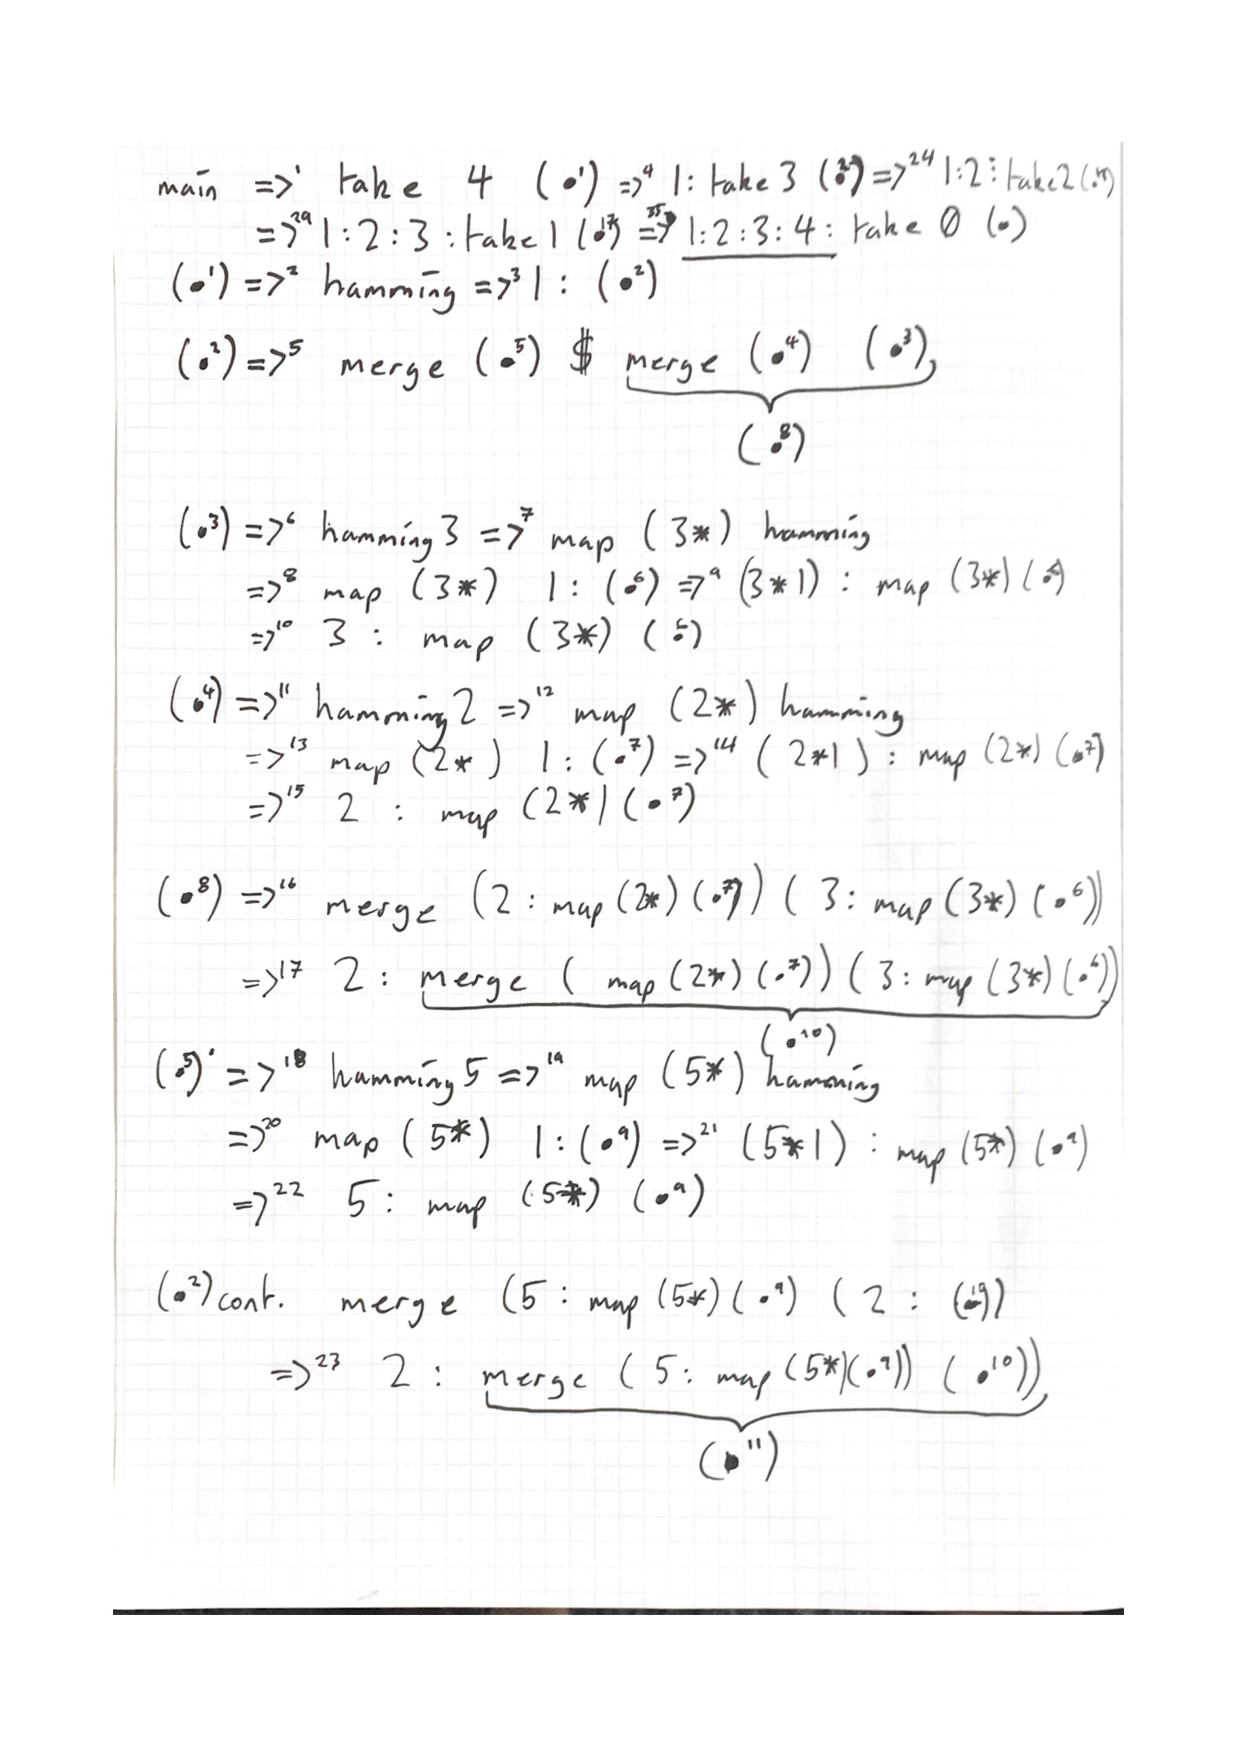
\includegraphics[scale=0.45]{HammingCycle1.pdf}
        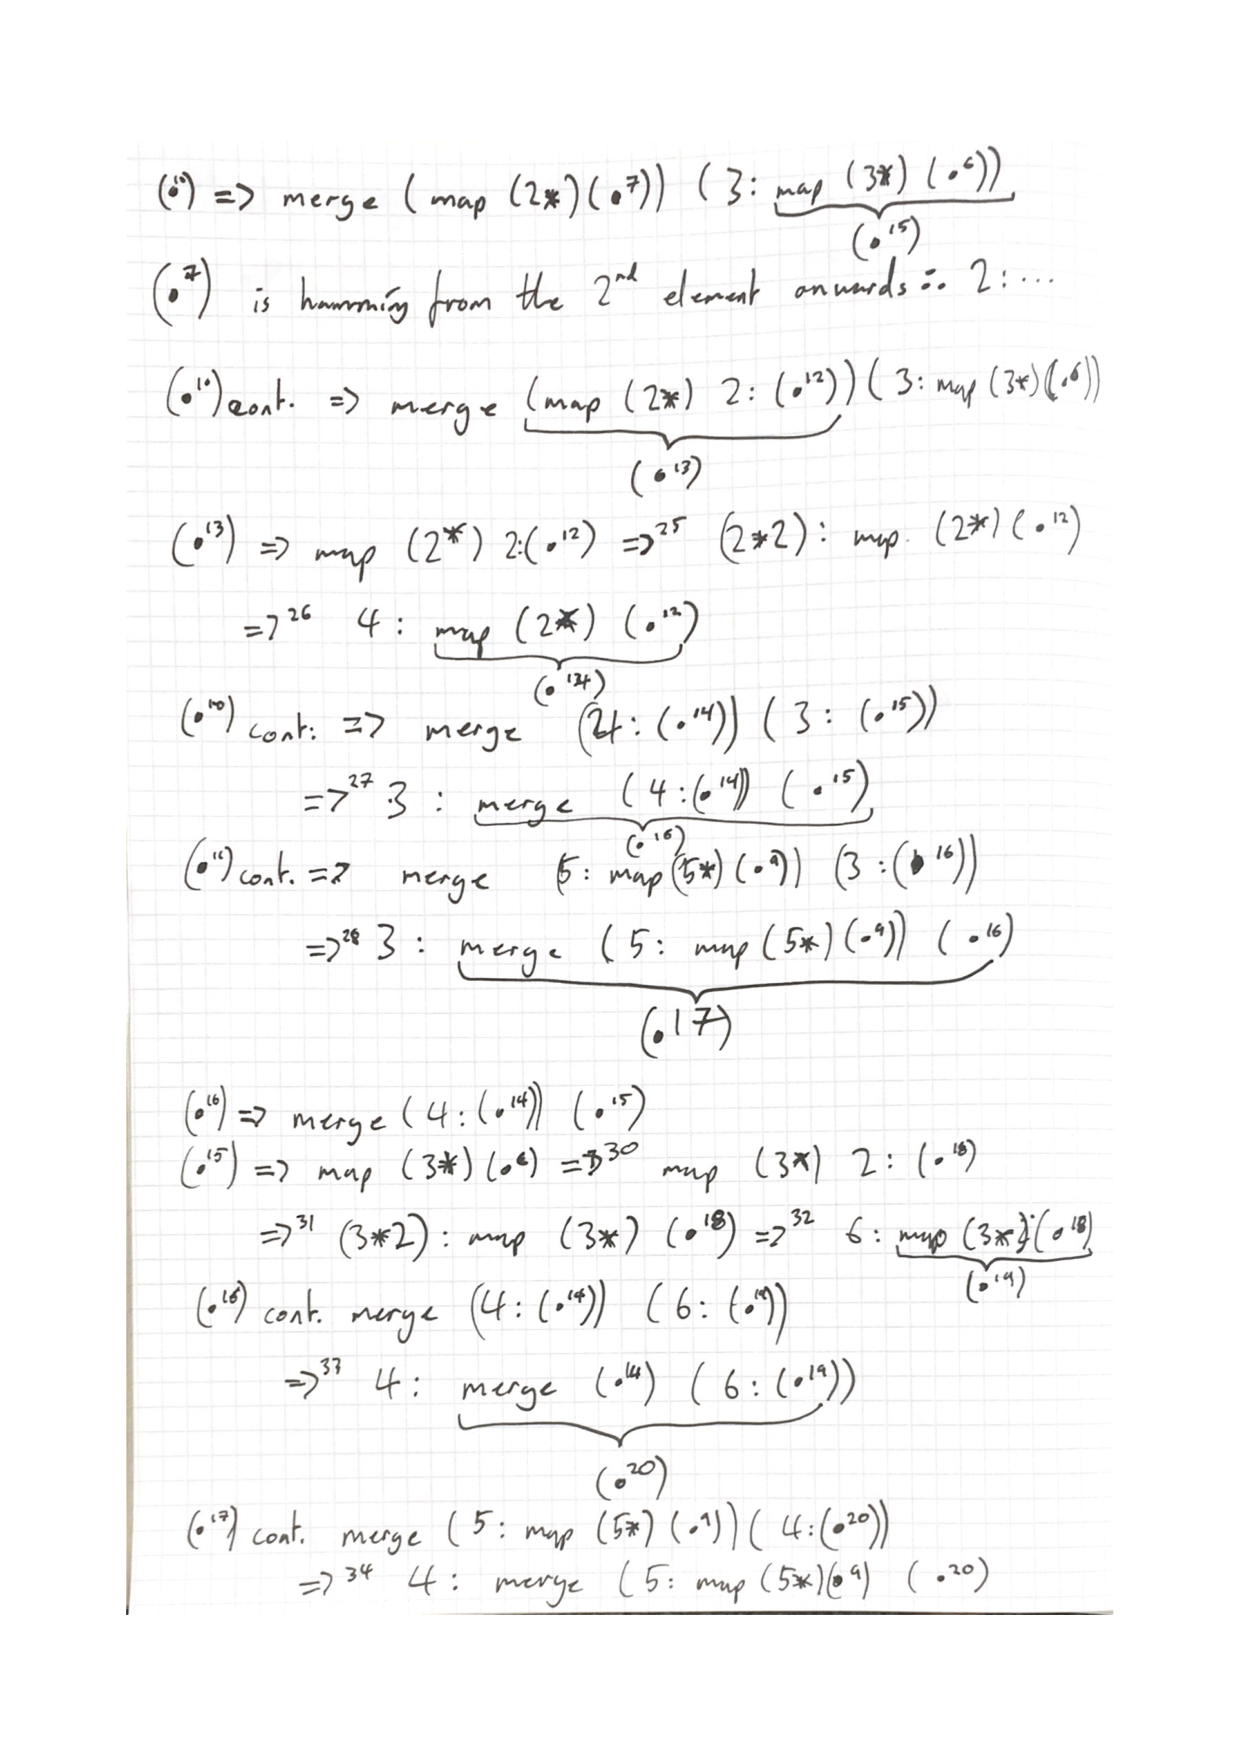
\includegraphics[scale=0.45]{HammingCycle2.pdf}
    \end{multicols}
\end{center}


\section{Task I.2 --- SpreadSheet Evaluator}
\subsection{Solution}
The following lines were added to evalCell to extend it to allow evaluation of sum and average expressions:
\lstinputlisting[language=Haskell, firstline=11, lastline=14]{reportCode.hs}
\par
To evaluate the sum between 2 cells a list of the cell values is created and then sum is used to add them all together.
To get all of the cell values to sum together, range is used to get a list of the cell references needed to be added together.
For each cell in that range evalCell is called upon it to get the cell value.
\medskip
\par
Average works in a similar way using the sum function previously defined to get the sum between the 2 cell references.
This value is then divided by the number of values added together, which can be found out by getting the length of the range between the 2 cells.
fromIntegral is used as / needs both values to be a Double but length will return an Integer.
\subsection{Weakness in the Evaluator}
The weakness in this evaluator is that if there is any cells that reference each other otherwise known as a circular reference.
If this occurs then the evaluator will hang as it tries to calculate an infinite loop.
One way to fix this would be to check for circular references before evaluating a sheet and if there is a circular reference throw an error.
This can be done by representing the sheet as a graph with each cell being a node and dependencies on other cells being edges.
Once this graph is generated you can perform cycle detection upon it to find circular references.
\par
Another approach that Microsoft Excel can use to compute circular references is to iterate over the sheet a number of times.
This can be necessary for some iterative functions to run.
You can calculate the value of the cell depending on the previous values and iterate up until a fixed number of iterations or until the values in the cells don't change.

\section{Task I.3 --- Skew Binary Random Access Lists}
\subsection{Solution}
The following lines were added to implment drop for Skew Binary Random Access Lists:
\lstinputlisting[language=Haskell, firstline=16, lastline=28]{reportCode.hs}
\par
drop takes the number of elements to drop (i) and the SBRAL to drop from and returns a new SBRAL with the first i elements dropped.
To begin with it checks the first tree in the list and compares the weight of the tree with number of elements to drop.
If the weight is \( \geq \) to the number of elements to drop, the first tree is ignored and then the subsequent number of elements are dropped from the remaining list recursively.
If the number to drop is less than the weight of the first tree it will try to drop i elements from the first tree and keep the rest of the list the same.
This is done via the helper function dropTree.
\par
dropTree has a couple of base cases for dropping a leaf node, if there are any number of nodes to drop it returns the empty list otherwise it will return a list with the leaf.
If a number of elements need to be dropped from a none leaf node then there is a series of guards that test for differing cases.
If 0 elements need to be dropped dropTree will repackage the weight and tree into a single element list and then return it.
If the number of nodes to drop is less than or equal to \( \frac{1}{2} \) the weight it is known that the root node needs to be dropped and potentially some elements in the right sub tree.
In this case the left sub tree doesn't need to be explored so it is repacked into a new RList and appended after the result of the recursive dropTree call.
If the number of nodes to drop is greater than \( \frac{1}{2} \) the weight then the right subtree can be completely disregarded and a number of elements need to be dropped from the left sub tree.

\subsection{Time Complexity}
The solution has the desired time complexity of  \( O(log\ n) \) just like lookup and update.
Like lookup and update, drop is implemented in a similar way therefore having the same time complexity.
\par
It will first find the correct tree it needs to drop elements from, by iterating through the list which is as long as the number of digits it takes to represent the number of elements stored as a skew binary number.
As with positional numbering systems the number of digits need is proportional to the size of the number by  \( log\ n \).
Therefore it takes \( O(log\ n) \) to find the correct tree it needs to drop elements from.
\par
To find the right element in the tree will take \( O(log\ n) \) as you need to go down the height of the tree making a decision at each level for which way to branch only once.
As its a binary tree the height is \( log\ n \).
Therefore it takes \( O(log\ n) \) to find the correct elements in the tree to stop dropping at.
\par
The overall worse case time complexity is \( log\ n + log\ n \) which can be shown as \( O(log\ n) \).

\subsection{Testing}
To test drop the following code was used:
\lstinputlisting[language=Haskell, firstline=48, lastline=59]{reportCode.hs}
\par
testDrop builds 2 SBRAL made entirely of 1s, one which is twice the size of the other, based upon the input number.
It then tries to drop that many elements from the large list meaning the 2 lists should be the same list in the end and test for that.
The other 2 functions implement a way to test dropping up to n elements from a list combines the result of all of those tests.

\section{Task I.4 --- Interval Arithmetic}
\subsection{Solution}
\subsubsection{Instance of Num}
The following lines were added to make Ivl an instance of Num:
\lstinputlisting[language=Haskell, firstline=30, lastline=37]{reportCode.hs}
\par
The definitions for +, - and * taken from wikipedia and implemented in Hakell - \url{https://en.wikipedia.org/wiki/Interval_arithmetic#Simple_arithmetic}.
While + and - are simple, * uses a list comprehension to find all possible bounds of multiplying the 2 intervals together and takes the smallest for the lower bound and largest for the upper bound.
\par
abs takes the interval and returns an interval between 0 and the absolute size of the original interval.
fromInteger simply takes a single value and returns a interval that is containing only that value.
signum returns an interval with each bound being the signum of each of the bounds.

\subsubsection{Instance of Fractional}
The following lines were added to make Ivl an instance of Fractional:
\lstinputlisting[language=Haskell, firstline=39, lastline=43]{reportCode.hs}
\par
Division is defined in the same way as multiplication in the Num instance using a list comprehension to create all possible bounds and taking the minimum and maximum.
fromRational is similar to fromInteger creating a interval of that rational number only.
recip doesn't have to be defined as the compiler can infer this definition from the both fromInteger and division but it has been added for clarity.
It simply divides 1 by the interval, this will use fromInteger and the previously defined divide.

\subsubsection{Defining \( \pm \) for Ivl}
The following lines were added to define the \( \pm \) function:
\lstinputlisting[language=Haskell, firstline=45, lastline=46]{reportCode.hs}
\par
\( \pm \) is an inline operator that will take 2 doubles and construct a symmetric interval around a the first double with the bounds being the size of the second double away from the middle.

\subsection{Testing}
A few tests were written and are in the code for intervals but the tests aren't complete and don't test all of the functions defined.






% \lstinputlisting[language=Haskell, firstline=0, lastline=23]{../Code/Hamming.hs}

\end{document}
